\begin{center}
\begin{tikzpicture}[x=1cm,y=1cm]
%\pgfresetboundingbox
\draw[use as bounding box, anchor = north west,draw=none] (-5.5,-3.25) rectangle (5.5,3.25);
\clip (-5.5,-3.25) rectangle (5.5,3.25);
\only<1->{\node[anchor =north west] (text) at (-5.25,3.25){\begin{minipage}{10.0cm}
\scriptsize Huang, B. \& von Lilienfeld, O.A.  \textit{arXiv} 1707.04146, ``The `DNA’of chemistry: Scalable quantum machine learning with amons", 2017.
\end{minipage}};}
\visible<1->{\node[anchor=west] (figure) at (-5.5,0){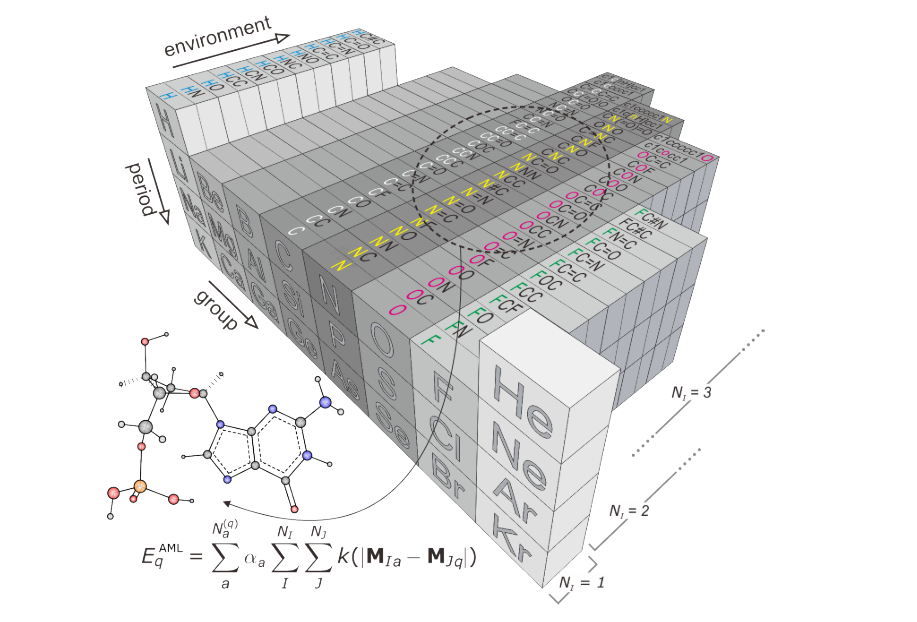
\includegraphics[width=5.5cm]{applications/images/oanatole1}};}
\visible<1->{\node[anchor=east] (figure) at (5.5,0){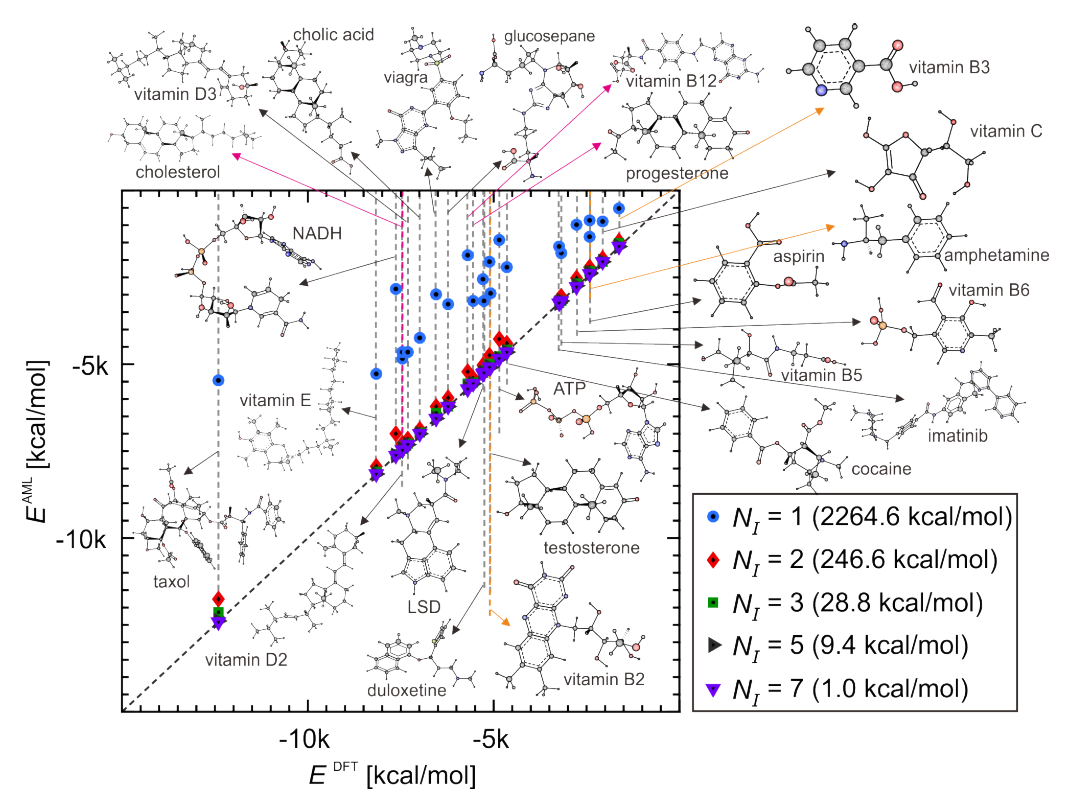
\includegraphics[width=6.5cm]{applications/images/oanatole}};}
\end{tikzpicture}
\end{center}